\documentclass[journal,12pt,twocolumn]{IEEEtran}
%
\usepackage{setspace}
%eghskljfnd
\usepackage{gensymb}
\usepackage{xcolor}
\usepackage{caption}
%\usepackage{subcaption}
%\doublespacing
\singlespacing

%\usepackage{graphicx}
%\usepackage{amssymb}
%\usepackage{relsize}
\usepackage[cmex10]{amsmath}
\usepackage{mathtools}
%\usepackage{amsthm}
%\interdisplaylinepenalty=2500
%\savesymbol{iint}
%\usepackage{txfonts}
%\restoresymbol{TXF}{iint}
%\usepackage{wasysym}
\usepackage{hyperref}
\usepackage{amsthm}
\usepackage{mathrsfs}
\usepackage{txfonts}
\usepackage{stfloats}
\usepackage{cite}
\usepackage{cases}
\usepackage{subfig}
%\usepackage{xtab}
\usepackage{longtable}
\usepackage{multirow}
%\usepackage{algorithm}
%\usepackage{algpseudocode}
%\usepackage{enumerate}
\usepackage{enumitem}
\usepackage{mathtools}
%\usepackage{iithtlc}
%\usepackage[framemethod=tikz]{mdframed}
\usepackage{listings}


%\usepackage{stmaryrd}

\usepackage{draftwatermark}
\SetWatermarkLightness{ 0.85 }
\SetWatermarkText{EE3900}
\SetWatermarkScale{1}
%\usepackage{wasysym}
%\newcounter{MYtempeqncnt}
\DeclareMathOperator*{\Res}{Res}
%\renewcommand{\baselinestretch}{2}
\renewcommand\thesection{\arabic{section}}
\renewcommand\thesubsection{\thesection.\arabic{subsection}}
\renewcommand\thesubsubsection{\thesubsection.\arabic{subsubsection}}

\renewcommand\thesectiondis{\arabic{section}}
\renewcommand\thesubsectiondis{\thesectiondis.\arabic{subsection}}
\renewcommand\thesubsubsectiondis{\thesubsectiondis.\arabic{subsubsection}}

%\renewcommand{\labelenumi}{\textbf{\theenumi}}
%\renewcommand{\theenumi}{P.\arabic{enumi}}

% correct bad hyphenation here
\hyphenation{op-tical net-works semi-conduc-tor}

\lstset{
language=Python,
frame=single, 
breaklines=true,
columns=fullflexible
}



\begin{document}
%

\theoremstyle{definition}
\newtheorem{theorem}{Theorem}[section]
\newtheorem{problem}{Problem}
\newtheorem{proposition}{Proposition}[section]
\newtheorem{lemma}{Lemma}[section]
\newtheorem{corollary}[theorem]{Corollary}
\newtheorem{example}{Example}[section]
\newtheorem{definition}{Definition}[section]
%\newtheorem{algorithm}{Algorithm}[section]
%\newtheorem{cor}{Corollary}
\newcommand{\BEQA}{\begin{eqnarray}}
        \newcommand{\EEQA}{\end{eqnarray}}
\newcommand{\define}{\stackrel{\triangle}{=}}
\bibliographystyle{IEEEtran}
%\bibliographystyle{ieeetr}
\providecommand{\nCr}[2]{\,^{#1}C_{#2}} % nCr
\providecommand{\nPr}[2]{\,^{#1}P_{#2}} % nPr
\providecommand{\mbf}{\mathbf}
\providecommand{\pr}[1]{\ensuremath{\Pr\left(#1\right)}}
\providecommand{\qfunc}[1]{\ensuremath{Q\left(#1\right)}}
\providecommand{\sbrak}[1]{\ensuremath{{}\left[#1\right]}}
\providecommand{\lsbrak}[1]{\ensuremath{{}\left[#1\right.}}
\providecommand{\rsbrak}[1]{\ensuremath{{}\left.#1\right]}}
\providecommand{\brak}[1]{\ensuremath{\left(#1\right)}}
\providecommand{\lbrak}[1]{\ensuremath{\left(#1\right.}}
\providecommand{\rbrak}[1]{\ensuremath{\left.#1\right)}}
\providecommand{\cbrak}[1]{\ensuremath{\left\{#1\right\}}}
\providecommand{\lcbrak}[1]{\ensuremath{\left\{#1\right.}}
\providecommand{\rcbrak}[1]{\ensuremath{\left.#1\right\}}}
\theoremstyle{remark}
\newtheorem{rem}{Remark}
\newcommand{\sgn}{\mathop{\mathrm{sgn}}}
\providecommand{\abs}[1]{\left\vert#1\right\vert}
\providecommand{\res}[1]{\Res\displaylimits_{#1}}
\providecommand{\norm}[1]{\lVert#1\rVert}
\providecommand{\mtx}[1]{\mathbf{#1}}
\providecommand{\mean}[1]{E\left[ #1 \right]}
\providecommand{\fourier}{\overset{\mathcal{F}}{ \rightleftharpoons}}
\providecommand{\ztrans}{\overset{\mathcal{Z}}{ \rightleftharpoons}}
%\providecommand{\hilbert}{\overset{\mathcal{H}}{ \rightleftharpoons}}
\providecommand{\system}{\overset{\mathcal{H}}{ \longleftrightarrow}}
%\newcommand{\solution}[2]{\textbf{Solution:}{#1}}
\newcommand{\solution}{\noindent \textbf{Solution: }}
\providecommand{\dec}[2]{\ensuremath{\overset{#1}{\underset{#2}{\gtrless}}}}
\numberwithin{equation}{section}
%\numberwithin{equation}{subsection}
%\numberwithin{problem}{subsection}
%\numberwithin{definition}{subsection}
\makeatletter
\@addtoreset{figure}{problem}
%\maketother
\let\StandardTheFigure\thefigure
%\renewcommand{\thefigure}{\theproblem.\arabic{figure}}
\renewcommand{\thefigure}{\theproblem}
%\numberwithin{figure}{subsection}
\def\putbox#1#2#3{\makebox[0in][l]{\makebox[#1][l]{}\raisebox{\baselineskip}[0in][0in]{\raisebox{#2}[0in][0in]{#3}}}}
\def\rightbox#1{\makebox[0in][r]{#1}}
\def\centbox#1{\makebox[0in]{#1}}
\def\topbox#1{\raisebox{-\baselineskip}[0in][0in]{#1}}
\def\midbox#1{\raisebox{-0.5\baselineskip}[0in][0in]{#1}}
\vspace{3cm}
\title{
    %\logo{
    Lab Report
    %}
    %	\logo{Octave for Math Computing }
}
%\title{
%	\logo{Matrix Analysis through Octave}{\begin{center}\includegraphics[scale=.24]{tlc}\end{center}}{}{HAMDSP}
%}
% paper title
% can use linebreaks \\ within to get better formatting as desired
%\title{Matrix Analysis through Octave}
%
%
% author names and IEEE memberships
% note positions of commas and nonbreaking spaces ( ~ ) LaTeX will not break
% a structure at a ~ so this keeps an author's name from being broken across
% two lines.
% use \thanks{} to gain access to the first footnote area
% a separate \thanks must be used for each paragraph as LaTeX2e's \thanks
% was not built to handle multiple paragraphs
%
\author{ Himanshu Kumar Gupta\\ AI21BTECH11012 %<-this  stops a space
     % stops a space
    %\thanks{J. Doe and J. Doe are with Anonymous University.}% <-this % stops a space
    %\thanks{Manuscript received April 19, 2005; revised January 11, 2007.}}
}
% note the % following the last \IEEEmembership and also \thanks - 
% these prevent an unwanted space from occurring between the last author name
% and the end of the author line. i.e., if you had this:
% 
% \author{....lastname \thanks{...} \thanks{...} }
%                     ^------------^------------^----Do not want these spaces!
%
% a space would be appended to the last name and could cause every name on that
% line to be shifted left slightly. This is one of those "LaTeX things". For
% instance, "\textbf{A} \textbf{B}" will typeset as "A B" not "AB". To get
% "AB" then you have to do: "\textbf{A}\textbf{B}"
% \thanks is no different in this regard, so shield the last } of each \thanks
% that ends a line with a % and do not let a space in before the next \thanks.
% Spaces after \IEEEmembership other than the last one are OK (and needed) as
% you are supposed to have spaces between the names. For what it is worth,
% this is a minor point as most people would not even notice if the said evil
% space somehow managed to creep in.
% The paper headers
%\markboth{Journal of \LaTeX\ Class Files,~Vol.~6, No.~1, January~2007}%
%{Shell \MakeLowercase{\textit{et al.}}: Bare Demo of IEEEtran.cls for Journals}
% The only time the second header will appear is for the odd numbered pages
% after the title page when using the twoside option.
% 
% *** Note that you probably will NOT want to include the author's ***
% *** name in the headers of peer review papers.                   ***
% You can use \ifCLASSOPTIONpeerreview for conditional compilation here if
% you desire.
% If you want to put a publisher's ID mark on the page you can do it like
% this:
%\IEEEpubid{0000--0000/00\$00.00~\copyright~2007 IEEE}
% Remember, if you use this you must call \IEEEpubidadjcol in the second
% column for its text to clear the IEEEpubid mark.
% \pagecolor{cyan!20!white}
\newcommand{\myvec}[1]{\ensuremath{\begin{pmatrix}#1\end{pmatrix}}}
% make the title area
\maketitle
%\newpage
\tableofcontents
%\renewcommand{\thefigure}{\thesection.\theenumi}
%\renewcommand{\thetable}{\thesection.\theenumi}
\renewcommand{\thefigure}{\theenumi}
\renewcommand{\thetable}{\theenumi}
%\renewcommand{\theequation}{\thesection}
\bigskip
\begin{abstract}
    This manual provides precedure of making a charger.
\end{abstract}
\section*{Aim of the experiment}
% \begin{enumerate}[label=\arabic*.,ref=\thesection.\theenumi]
    In this experiment we made a charger of output 5V by using the circuit given in the report.
    we used different equipments and electrical devices to change the input of 220V AC to 5V DC.
\section*{Material required}
\begin{enumerate}[label=\arabic*.,ref=\thesection.\theenumi]
    \item Solderless Breadboard
    \item Printed Circuit board
    \item Transformer(12-0-12)
    \item 4 IN4007 diode
    \item capacitor($100\mu$ F)
    \item 7805 Regulator
    \item Output point
    \item AC cable with a plug.
    \item Multi-meter
    \item Cathode-ray oscilloscope
    \item USB cable
\end{enumerate}
\section*{Circuit explanation}
The transformer steps down the 230V AC main supply to 12V AC. Note that these are RMS voltages. The peak voltage will thus be $12\sqrt{2} \approx 18V$. The transformed voltage is given by
\begin{align}
v(t) &= 12\sqrt{2}\sin(100\pi t + \phi) V
\end{align}
\section*{Procedure}
After collecting all the material requied we started arranging the tansistor, capacitor and diode in a proper manner as shown in circuit. Firsty we connected transformer so as to convert 230V to 12V.Then after fitting remaining material in breadboard we measured the output using multimeter.
Since we had got the correct output ie. 5V so we removed the electrical equipments from the breadboard and arranged in the POC in the same arrangement as it was in breadboard.After that we did soledring using solder iron and solder wire.Since the remaining wire was harmful and of no use so we removed them.
\begin{figure}
\centering
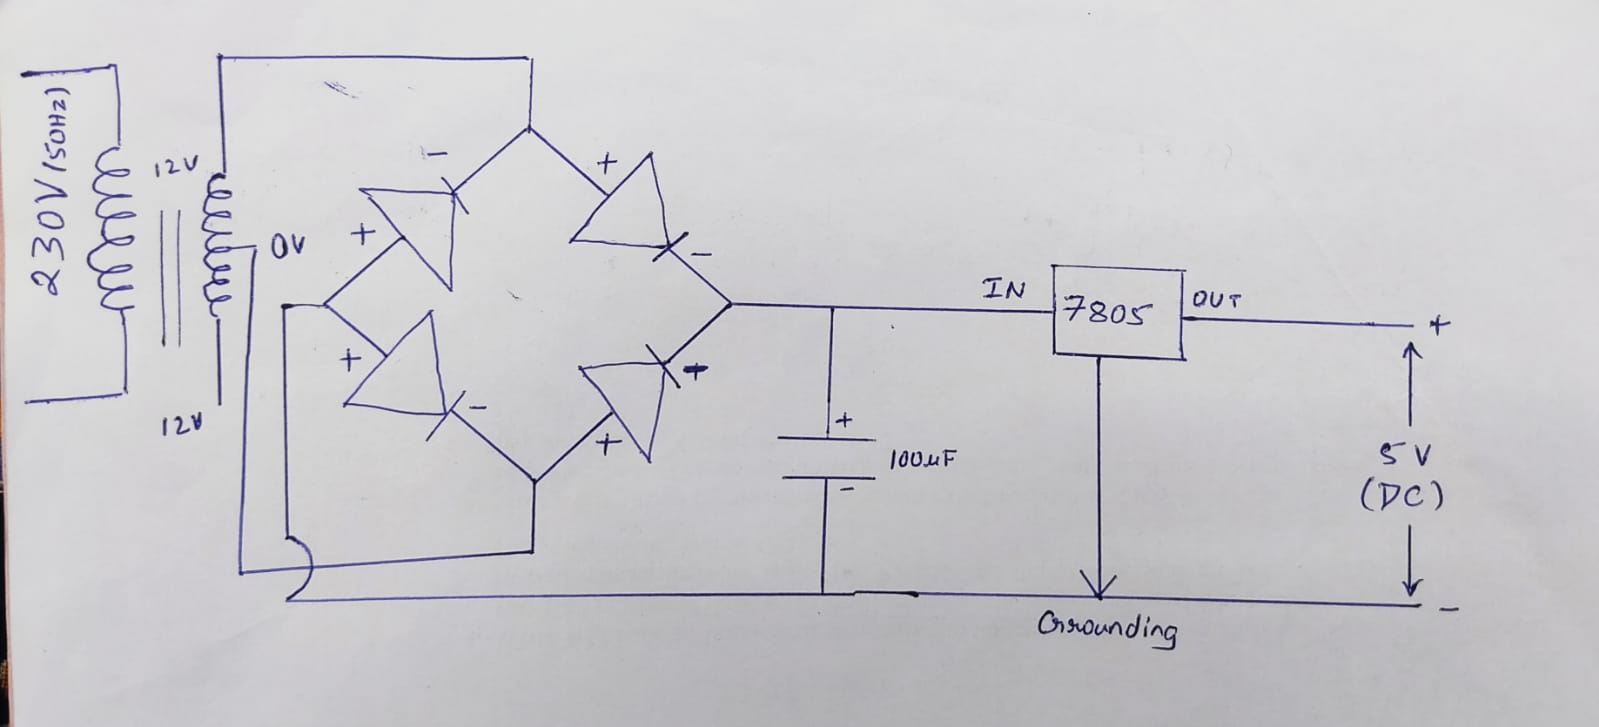
\includegraphics[width=\columnwidth]{./figs/p0.jpeg}
\caption*{fig.1 Circuit diagram of charger}
\label{output_1}
\end{figure}
\section*{Observatrion}
We have checked that the output we are getting is 5V so to verify it again we again checked it with cathode ray oscilloscope (CRO).Again we got the same reading as multimeter. after this we measured the voltage across half wave rectifire whose reult is ther in fig.2.
\begin{figure}
    \centering
    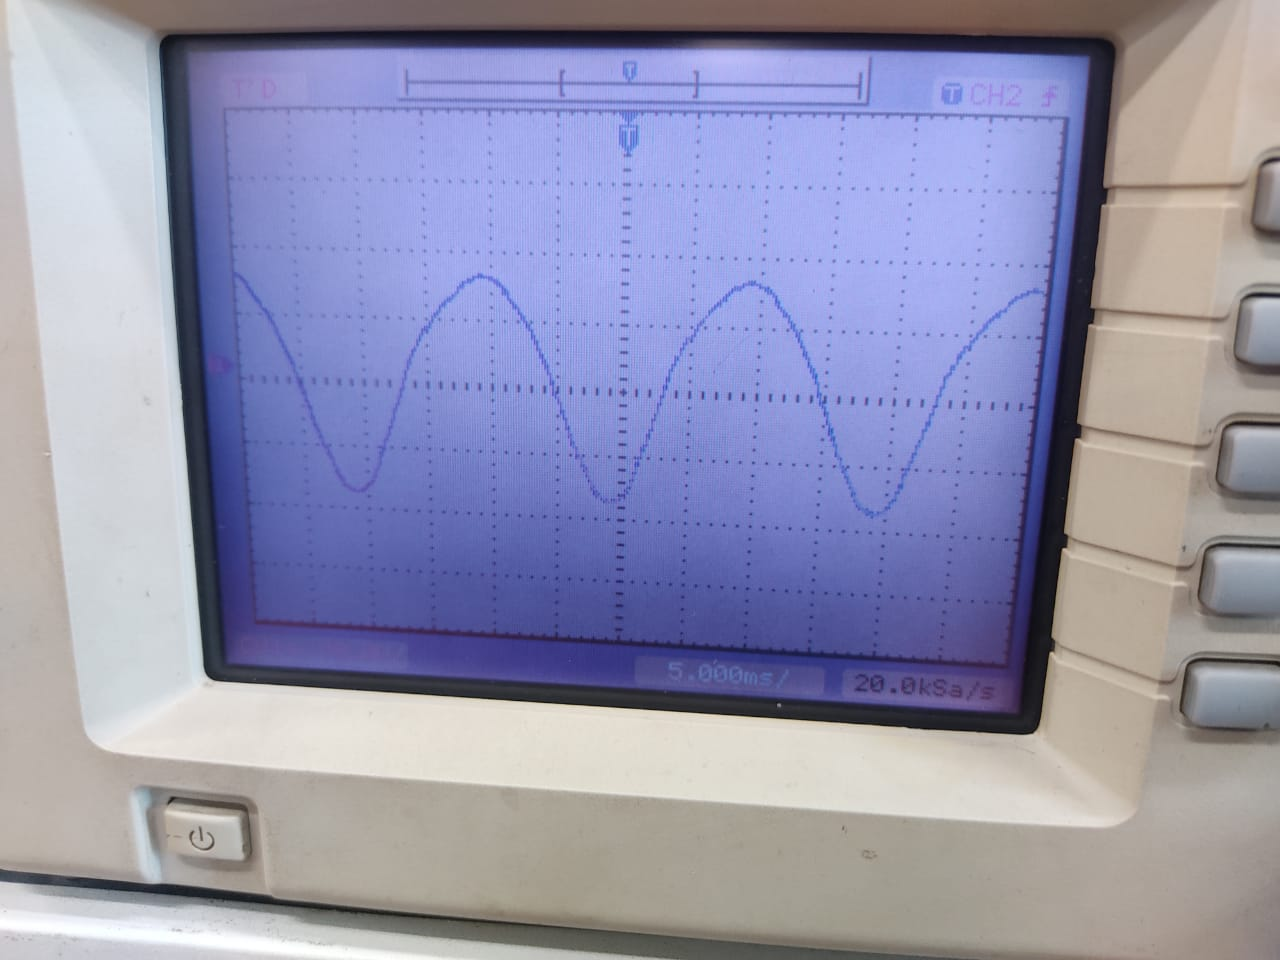
\includegraphics[width=\columnwidth]{./figs/p2.jpeg}
    \caption*{fig.2 CRO output of transformer}
    \label{output_2}
\end{figure}
\section*{Result}
    Now after doing all the observations we have became ready to charge our Mobile phone. For that we attached a usb (Type C) cabel to the output point.On connecting the
    USB cable to the mobile phone and switching on the
    main supply to which the transformer is connected,
    we can see that the mobile phone is getting charged
    successfully.
    \begin{figure}
        \centering
        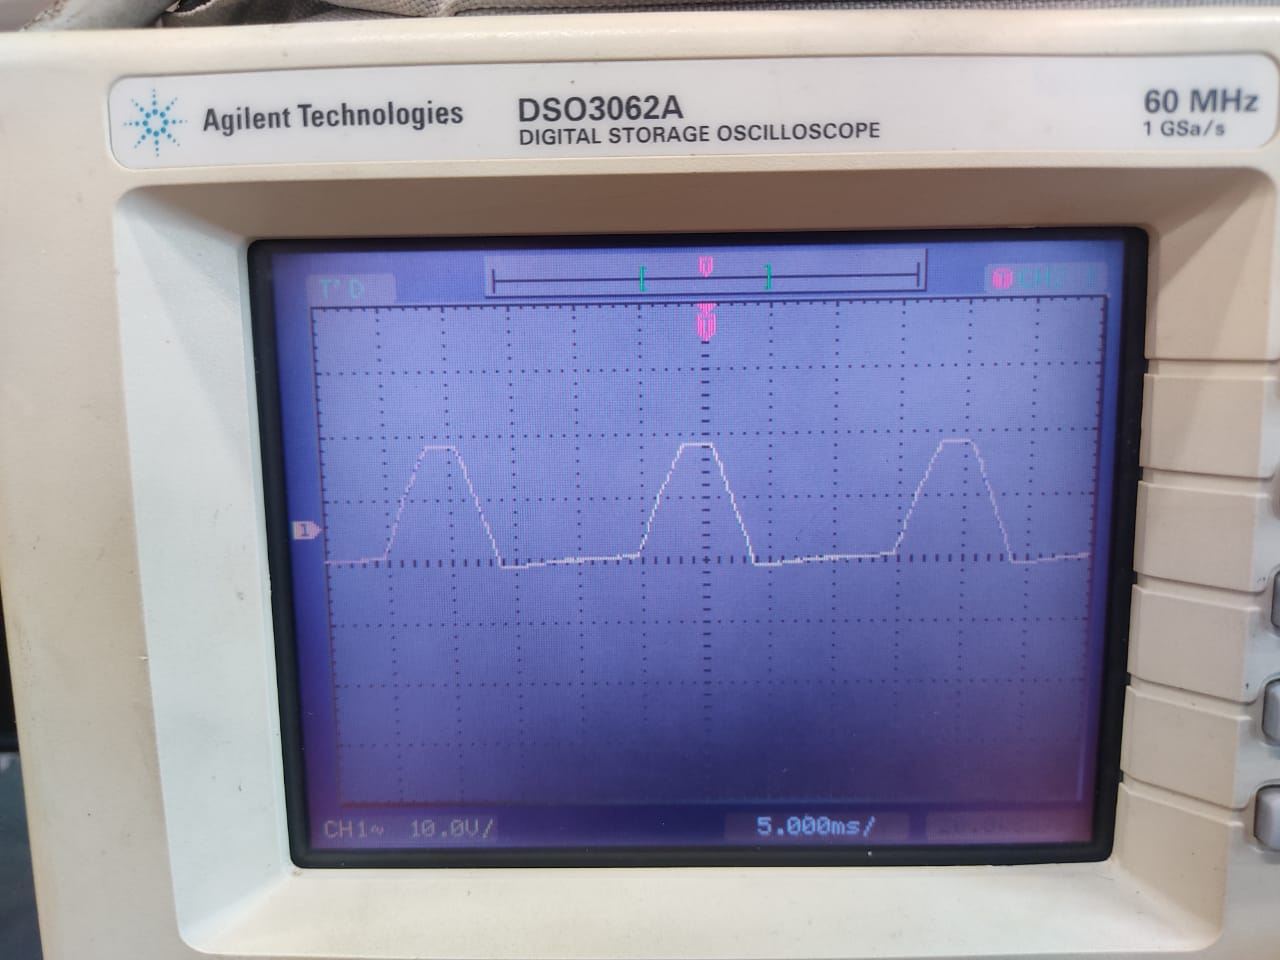
\includegraphics[width=\columnwidth]{./figs/p1.jpeg}
        \caption*{fig.3 CRO output of half wave rectified voltage across diode}
        \label{output_3}
    \end{figure}
    \begin{figure}
        \centering
        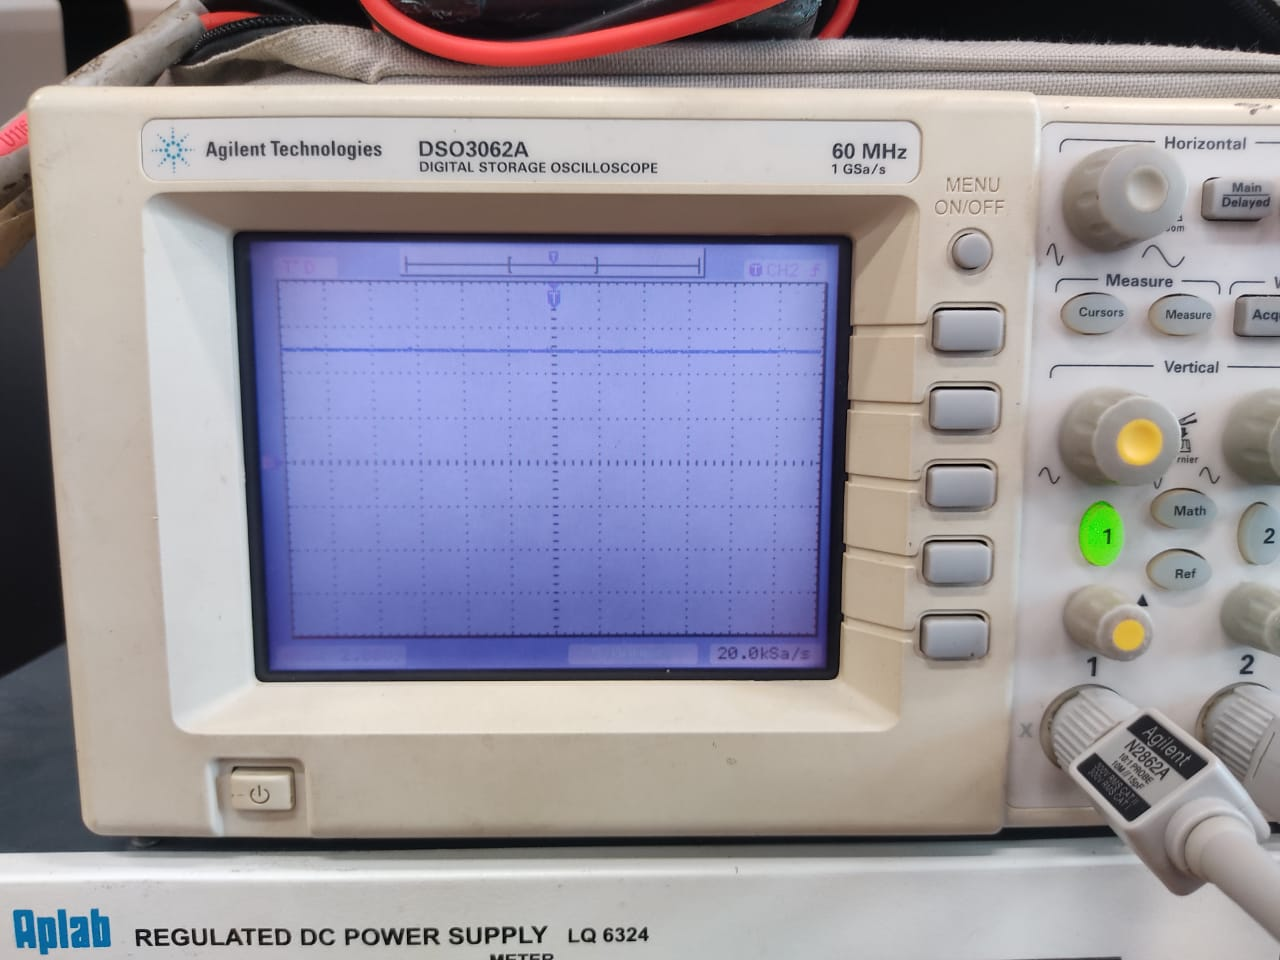
\includegraphics[width=\columnwidth]{./figs/p3.jpeg}
        \caption*{fig.4 CRO reding of main output of charger}
        \label{output_4}
    \end{figure}
\end{document}a
